En esta sección, revisamos
brevemente~\citep{choksi_partial_2022,salgado_classical_2022} los
conceptos asociados a un problema de valor de frontera y su solución.
Luego, derivaremos la ecuación de advección-difusión unidimensional
según~\citep{leveque_numerical_1992}.
Finalmente, mostramos el método de las líneas para convertir nuestra
ecuación de interés en un sistema de ecuaciones diferenciales
ordinarias.

\section{GENERALIDADES}

\begin{definition}[Ecuación diferencial parcial]
    Es una ecuación que involucra una \emph{función desconocida} $u$
    y sus derivadas parciales junto con las variables independientes.
    Se escribe como
    \begin{equation}
        \boxed{
            F\left(
            \text{variables independientes},
            u,
            \text{derivadas de $u$}
            \right)
            =0
        }.\label{eq:pde}
    \end{equation}
\end{definition}

\begin{definition}[Solución de una ecuación diferencial parcial]
    Sea $\Omega\subset\mathbb{R}^{d}$ un conjunto abierto y conexo.
    Una \emph{solución} es una función $u\colon\Omega\to\mathbb{R}$
    que satisface~\eqref{eq:pde} para cualquier $x\in\Omega$.
\end{definition}

\begin{definition}[Condiciones auxiliares]
    Sea $\Omega\subset\mathbb{R}^{d}$ un conjunto abierto y conexo.
    Una \emph{condición auxiliar} en una solución general es una
    igualdad que especifica el valor de la función desconocida en un
    subconjunto de $\Omega$.
\end{definition}

\begin{definition}[Problema de valor inicial]
    Sea
    \begin{math}
        u\colon
        \Omega\times\left[0,T\right]\subset
        \mathbb{R}^{d}\times\mathbb{R}\to
        \mathbb{R}
    \end{math}
    una solución de~\eqref{eq:pde}.
    Un \emph{problema de valor inicial} es una ecuación diferencial
    junto con un conjunto de condiciones auxiliares que especifican
    la solución y/o sus derivadas en $t=0$.
\end{definition}

\begin{definition}[Problema de valor de frontera]
    Sea
    \begin{math}
        u\colon
        \Omega\subset
        \mathbb{R}^{d}\to
        \mathbb{R}
    \end{math}
    una solución de~\eqref{eq:pde}.
    Un \emph{problema de valor de frontera} es una ecuación
    diferencial junto con un conjunto de condiciones auxiliares que
    especifican la solución y/o sus derivadas en $\partial\Omega$.
\end{definition}

\begin{definition}[Dominio]
    Un dominio $\Omega$ es un subconjunto de $\mathbb{R}^{d}$ abierto
    y conexo que tiene frontera lineal a trozos de clase $C^{1}$.
\end{definition}

\begin{theorem}[Identidades integrales]
    Sea
    \begin{math}
        \Omega\subset
        \mathbb{R}^{d}
    \end{math}
    un dominio acotado con frontera suficientemente suave
    y
    \begin{math}
        n\colon
        \partial\Omega\to
        \mathbb{R}^{d}
    \end{math}
    normal unitario hacia afuera.
    Se cumplen
    \begin{description}
        \item[Integración por partes.]

            Si $u,v\in C^{1}\left(\overline{\Omega}\right)$, entonces
            \begin{equation*}
                \int_{\Omega}\diffp{u\left(x\right)}{x_{i}}
                v\left(x\right)\dl x=
                \int_{\partial\Omega}
                u\left(x\right)
                v\left(x\right)
                n\left(x\right)\cdot
                e_{i}
                \dl{S\left(x\right)}-
                \int_{\Omega}u\left(x\right)
                \diffp{v\left(x\right)}{x_{i}}
                \dl x.
            \end{equation*}

        \item[Primera identidad de Green.]
            Si $v\in C^{1}\left(\overline{\Omega}\right)$ y
            $w\in C^{2}\left(\overline{\Omega}\right)$, entonces
            \begin{equation*}
                \int_{\Omega}\nabla v\left(x\right)\cdot
                w\left(x\right)\dl x=
                -\int_{\Omega}
                v\left(x\right)
                \Delta w\left(x\right)
                \dl x+
                \int_{\partial\Omega}
                v\left(x\right)
                \diffp{w\left(x\right)}{n}
                \dl{S\left(x\right)},
            \end{equation*}
            donde
            \begin{math}
                \diffp{w\left(x\right)}{n}=
                n\left(x\right)\cdot
                \nabla w\left(x\right)
            \end{math}.

        \item[Segunda identidad de Green.]

            Si $v,w\in C^{2}\left(\overline{\Omega}\right)$, entonces
            \begin{equation*}
                \int_{\Omega}
                \left(
                v\left(x\right)
                \Delta w\left(x\right)-
                \Delta v\left(x\right)
                w\left(x\right)
                \right)
                \dl x=
                \int_{\partial\Omega}
                \left(
                v\left(x\right)
                \diffp{w}{n}\left(x\right)-
                \diffp{v}{n}\left(x\right)
                w\left(x\right)
                \right)
                \dl{S\left(x\right)}.
            \end{equation*}

        \item[]

            Si $v\in C^{1}\left(\overline{\Omega};\mathbb{R}^{d}\right)$ y
            $w\in C^{1}\left(\overline{\Omega}\right)$, entonces
            \begin{equation*}
                \int_{\Omega}\nabla\cdot v\left(x\right)
                w\left(x\right)
                \dl x=
                \int_{\partial\Omega}
                v\left(x\right)\cdot
                n\left(x\right)
                w\left(x\right)
                \dl{S\left(x\right)}-
                \int_{\Omega}
                v\left(x\right)\cdot
                \nabla w\left(x\right)
                \dl x.
            \end{equation*}
    \end{description}
\end{theorem}

\begin{definition}[Clasificación]
    Sea la ecuación diferencial parcial de segundo orden de
    coeficientes constantes
    \begin{math}
        \mathcal{D}u\left(x\right)=
        f\left(x\right)
    \end{math},
    \begin{math}
        m\in\mathbb{N}
    \end{math}
    y
    \begin{math}
        x\in\mathbb{R}^{m}
    \end{math}.

    \begin{align*}
        \mathcal{D}
        u\left(x\right) & =
        \sum_{i,j=1}^{m}
        \diffp[2]{v\left(x\right)}{x_{i}x_{j}}+
        \sum_{i=1}^{m}
        b_{i}
        \diffp{v\left(x\right)}{x_{i}}+
        cu\left(x\right)    \\
                        & =
        A\colon D^{2}u\left(x\right)+
        b\cdot\nabla u\left(x\right)+
        cv\left(x\right),
    \end{align*}
    donde $A=\left[a_{ij}\right]\in\mathbb{R}^{m\times m}$,
    \begin{math}
        b={\left[b_{i}\right]}^{T}\in\mathbb{R}^{m}
    \end{math},
    \begin{math}
        D^{2}u\left(x\right)
    \end{math}
    es la matriz hessiana de $u$ en el $x$,
    \begin{math}
        \nabla u\left(x\right)
    \end{math}
    es su gradiente en el mismo punto
    y
    \begin{equation*}
        \forall A,B\in\mathbb{R}^{m\times m}:\quad
        A\colon B=\operatorname{tr}\left(AB^{T}\right).
    \end{equation*}

    \begin{description}
        \item[Elíptico:]

            Si $\sigma\left(A\right)\subset\mathbb{R}_{+}$ o
            $\sigma\left(A\right)\subset\mathbb{R}_{-}$.

        \item[Parabólico:]

            Si $A$ contiene exactamente $m-1$ valores propios
            positivos o negativos y cero es un valor propio de
            multiplicidad uno.

        \item[Hiperbólico:]

            Si $A$ tiene $m-1$ valores propios positivos o negativos,
            y el restante es distinto de cero y de signo opuesto.

        \item[Ultra parabólico:]

            Si cero es un valor propio múltiple y todos los restantes
            tienen el mismo signo.

        \item[Ultra hiperbólico:]

            Si cero no es un valor propio y hay más de un valor
            propio positivo y más de un valor propio negativo.
    \end{description}
\end{definition}

\subsection{Leyes de conservación}

Sea
\begin{math}
    u\left(x,t\right)
\end{math}
la función concentración o densidad de alguna sustancia química.

\subsection{Aproximaciones de diferencias finitas de las derivadas}

Si $u\colon\mathbb{R}^d\to\mathbb{R}$ es una función suficientemente
suave y
\begin{equation*}
    \forall i=1,\dotsc d:\quad
    \diffp{u\left(x\right)}{x_{i}}=
    \lim\limits_{h\to0}
    \dfrac{
        u\left(x+he_{i}\right)-
        u\left(x\right)}{h},
\end{equation*}

donde $e_{i}$ es el $i$-ésimo vector de la base canónica de
$\mathbb{R}^d$.

El método de las diferencias finitas surge al aproximar la derivada
de una función por una expresión de diferencias de valores de esta en
ciertos puntos discretos cercanos, y así, convertimos una ecuación
diferencial en un sistema finito de ecuaciones algebraicas que puede
ser resuelto en la computadora.
La elección de esta ``diferencia finita'' debería ser

\begin{description}
    \item[Consistente:]

        La aproximación sea tan precisa como sea posible y encontrar
        una aproximación de diferencia finita de las derivadas que
        sea consistente con el orden más alto posible.

    \item[Estable:]

        No solo con respecto a perturbaciones de los datos, sino
        en las versiones discretas de las mismas normas en las que la
        solución al problema continuo posee sus propias propiedades
        estabilidad.
\end{description}

% TODO: p. 103. [Hundsdorfer]
Una condición necesaria para la estabilidad es que el dominio de
dependencia de la ecuación diferencial parcial esté contenida en el
dominio de dependencia numérico, y en los problemas lineales es
conocido como

% TODO: p. 46 [Lax].
\begin{theorem}[Teorema de Equivalencia de Lax-Richtmyer]
    Un problema de valor inicial bien planteado y una aproximación de
    diferencia finita que satisface la condición de consistencia y
    estabilidad es una condición necesaria y suficiente para la
    convergencia.
\end{theorem}

\begin{figure}[ht!]
    \centering
    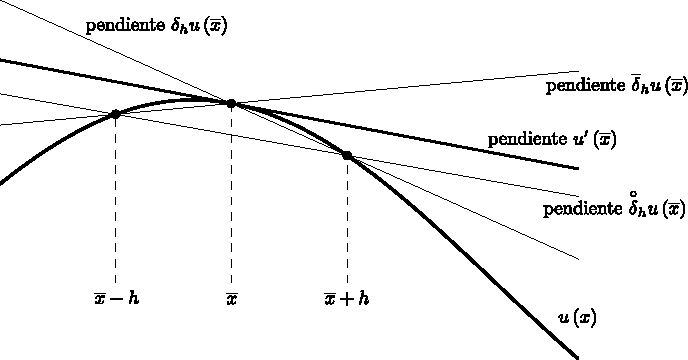
\includegraphics[width=.5\paperwidth]{E_IMAGENES/1_Capitulo2/finite_difference.pdf}
    \caption{
        Ilustración de los operadores de diferencias finitas usuales.
        Adaptado de~\citep{leveque_numerical_1992}.
    }
\end{figure}

Ahora, presentaremos algunas definiciones generales acerca de las
discretizaciones que nos permitirá estudiar la consistencia y
estabilidad de los esquemas venideros.

\begin{definition}[Malla uniforme]
    Sean $N\in\mathbb{N}$.
    El tamaño de la malla es
    \begin{math}
        h=\dfrac{1}{N+1}
    \end{math} y la malla uniforme es
    \begin{equation*}
        \mathbb{Z}^{d}_{h}\coloneqq
        \left\{
        hz\in\mathbb{R}^{d}\mid
        z\in\mathbb{Z}^{d}
        \right\}.
    \end{equation*}
\end{definition}

\begin{definition}[Conjunto de funciones malla]
    \begin{math}
        \emptyset\neq\mathcal{G}_{h}\subset\mathbb{Z}^{d}_{h}
    \end{math}
    es un dominio malla.
    Los puntos $x\in\mathcal{G}_{h}$ son los nodos o puntos de la malla.
    Se define el conjunto de funciones malla sobre $\mathcal{G}_{h}$
    como
    \begin{equation*}
        \mathcal{V}
        \left(\mathcal{G}_{h}\right)\coloneqq
        \left\{
        v\mid v\colon\mathcal{G}_{h}\to\mathbb{R}
        \right\}.
    \end{equation*}
    Además,
    \begin{math}
        \forall v\in\mathcal{V}\left(\mathcal{G}_{h}\right):
        \forall hi\in\mathcal{G}_{h}:
        v_{i}=v\left(hi\right)
    \end{math}.
\end{definition}

\begin{definition}[Espacio $\mathcal{V}_{0}\left(\overline{\Omega}_{h}\right)$]
    Sean
    \begin{math}
        \Omega=
        {\left(0,1\right)}^{d}
    \end{math},
    \begin{math}
        N\in\mathbb{N}
    \end{math},
    \begin{math}
        h=\dfrac{1}{\left(N+1\right)}
    \end{math}
    y
    \begin{math}
        \overline{\Omega}_{h}=
        \overline{\Omega}\cap
        \mathbb{Z}^{d}_{h}
    \end{math}.
    \begin{equation*}
        \mathcal{V}_{0}\left(\overline{\Omega}_{h}\right)\coloneqq
        \left\{
        v\in\mathcal{V}\left(\overline{\Omega}_{h}\right)
        \right\}
    \end{equation*}
\end{definition}

\begin{definition}[Operador diferencia finita]
    La aplicación
    \begin{equation*}
        \mathcal{F}_{h}\colon
        \mathcal{V}\left(\mathbb{Z}^{d}_{h}\right)\to
        \mathcal{V}\left(\mathbb{Z}^{d}_{h}\right)
    \end{equation*}
    es llamada \emph{operador de diferencia finita} sii
    \begin{equation*}
        \forall x\in\mathbb{Z}^{d}_{h}:
        \left(\mathcal{F}_{h}u\right)\left(x\right)=
        \sum_{e\in S}
        a_{e}\left(x,h\right)
        \left(\mathcal{S}_{e}v\right)
        \left(x\right),
    \end{equation*}
    donde $S\subset\mathbb{Z}^{d}_{h}$ es finito y $0\in S$.
\end{definition}

Sean
\begin{math}
    \left(
    \mathbb{V},
    {\left\|\cdot\right\|}_{\mathbb{V}}
    \right)
\end{math},
\begin{math}
    \left(
    \mathbb{F},
    {\left\|\cdot\right\|}_{\mathbb{F}}
    \right)
\end{math}
y
\begin{math}
    \left(
    \mathbb{G},
    {\left\|\cdot\right\|}_{\mathbb{G}}
    \right)
\end{math}
tres espacios normados, donde el primero es de funciones definidas
sobre $\overline{\Omega}={\left[0,1\right]}^{d}$.
Encuentre un $u\in\mathbb{V}$ tal que
\begin{equation*}
    \begin{cases}
        Lu=f,     & \text{ in }\Omega,         \\
        \ell u=g, & \text{ in }\partial\Omega,
    \end{cases}
\end{equation*}
donde $L$ y $\ell$ son operadores diferenciables.
El primero está asociado con la ecuación diferencial y el segundo con
las condiciones de frontera.
Las funciones $f\colon\Omega\to\mathbb{R}$ y $g\colon\partial\Omega\to\mathbb{R}$
son elementos de $\mathbb{F}$ y $\mathbb{G}$, respectivamente.

Encuentre un $w\in\mathcal{V}\left(\overline{\Omega}_{h}\right)$ tal
que
\begin{equation*}
    \begin{cases}
        L_{h}w=f_{h},    & \text{ in }\Omega^{I}_{h}, \\
        \ell_{h}w=g_{h}, & \text{ in }\Omega^{B}_{h},
    \end{cases}
\end{equation*}
donde $L_{h}$ y $\ell_{h}$ son operadores de diferencias finitas,
\begin{math}
    \Omega^{I}_{h}
\end{math}
y
\begin{math}
    \Omega^{B}_{h}
\end{math}
son los puntos malla interiores y frontera, respectivamente.

Sea un dominio espacio-temporal contenido en $\mathbb{R}^{d+1}$.

\begin{definition}[Dominio malla espacio-temporales]
    Sean
    \begin{math}
        \Omega=
        {\left(0,1\right)}^{d}
    \end{math},
    $T>0$, $K,N\in\mathbb{N}$.
    \begin{equation*}
        \overline{\mathcal{C}}^{\tau}_{h}\coloneqq
        \overline{\Omega}_{h}
        \times
        {\left[0,T\right]}_{\tau}=
        \left\{
        \left(x,t_{k}\right)\mid
        x\in\overline{\Omega}_{h},
        t_{k}=k\tau,
        k=0,\dotsc, K
        \right\}.
    \end{equation*}
\end{definition}

\begin{definition}[Interior discreto de $\overline{\mathcal{C}}^{\tau}_{h}$]
    \begin{equation*}
        \overline{\mathcal{C}}^{\tau}_{h}\coloneqq
        \Omega_{h}\times
        {\left(0,T\right)}_{\tau}.
    \end{equation*}
\end{definition}

\begin{definition}[Frontera lateral discreta]
    \begin{equation*}
        \partial_{L}
        \mathcal{C}^{\tau}_{h}\coloneqq
        \partial\Omega_{h}\times
        {\left[0,T\right]}_{\tau}.
    \end{equation*}
\end{definition}

\begin{definition}[Frontera parabólica discreta]
    \begin{equation*}
        \partial_{p}
        \mathcal{C}^{\tau}_{h}\coloneqq
        \overline{\Omega}_{h}\times
        \left\{0\right\}\cup
        \partial_{L}
        \mathcal{C}^{\tau}_{h}.
    \end{equation*}
\end{definition}

\begin{definition}[Espacio de funciones malla espacio-temporales]
    Sea $\mathcal{C}^{\tau}_{h}$ un dominio malla espacio-temporales.
    El espacio de funciones
    \begin{align*}
        \mathcal{V}
        \left(
        \overline{\mathcal{C}}^{\tau}_{h}
        \right) & =
        \left\{
        v\mid\overline{\mathcal{C}}^{\tau}_{h}\to\mathbb{R}
        \right\}.   \\
        \mathcal{V}
        \left(
        \mathcal{C}^{\tau}_{h}
        \right) & =
        \left\{
        v\mid\mathcal{C}^{\tau}_{h}\to\mathbb{R}
        \right\}.   \\
        \mathcal{V}
        \left(
        \partial_{L}\mathcal{C}^{\tau}_{h}
        \right) & =
        \left\{
        v\mid\partial_{L}\mathcal{C}^{\tau}_{h}\to\mathbb{R}
        \right\}.   \\
        \mathcal{V}_{0}
        \left(
        \overline{\mathcal{C}}^{\tau}_{h}
        \right) & =
        \left\{
        v\in\mathcal{V}\left(\overline{\mathcal{C}}^{\tau}_{h}\right)\mid
        v\left(x,t\right)=0,
        \forall\left(x,t\right)\in\partial_{L}\mathcal{C}^{\tau}_{h}
        \right\}.   \\
        \mathcal{V}
        \left(
        \overline{\Omega}_{h}
        \right) & =
        \left\{
        v^{k}\mid
        v\in
        \mathcal{V}
        \left(
        \overline{\mathcal{C}}^{\tau}_{h}
        \right),
        v^{k}\left(x\right)=
        v\left(x,k\tau\right)
        \forall x\in\overline{\Omega}_{h}
        \right\}
    \end{align*}
\end{definition}

Los espacios de funciones malla espacio-temporales pueden
identificarse como un espacio de funciones de valor función malla
espacial, o sea

\begin{align*}
    \mathcal{V}
    \left(
    \overline{\mathcal{C}}^{\tau}_{h}
    \right) & =
    \mathcal{V}
    \left(
    \left[0,T\right]_{\tau};
    \mathcal{V}\left(\overline{\Omega}_{h}\right)
    \right)=
    {\left(\mathcal{V}\left(\overline{\Omega}_{h}\right)\right)}^{K+1}. \\
    \mathcal{V}_{0}
    \left(
    \overline{\mathcal{C}}^{\tau}_{h}
    \right) & =
    \mathcal{V}
    \left(
    \left[0,T\right]_{\tau};
    \mathcal{V}_{0}\left(\overline{\Omega}_{h}\right)
    \right).
\end{align*}

\begin{definition}
    Sean
    \begin{math}
        d\in\left\{,12\right\}
    \end{math},
    \begin{math}
        p\in\left[1,\infty\right]
    \end{math}
    y
    \begin{math}
        q\in\left[1,\infty\right)
    \end{math}.

    \begin{align*}
        {\left\|v\right\|}_{L^{q}_{\tau}\left(L^{p}_{h}\right)}
         & =
        {\left(
        \tau\sum_{k=1}^{K}
        \left\|v^{k}\right\|^{q}_{L^{p}_{h}}
        \right)}^{\frac{1}{q}}. \\
        {\left\|v\right\|}_{L^{\infty}_{\tau}\left(L^{p}_{h}\right)}
         & =
        \max^{K}_{k=0}
        {\left\|v^{k}\right\|}_{L^{p}_{h}}.
    \end{align*}
\end{definition}

\begin{definition}[Número de Courant]
    Sea $\overline{\mathcal{C}}^{\tau}_{h}$ una malla espacio-temporal.
    El número de Courant parabólico es
    \begin{equation*}
        \mu=
        \dfrac{\tau}{h^{2}}.
    \end{equation*}
\end{definition}

\begin{definition}[Estabilidad condicional]
    Decimos que un método de diferencia finita es \emph{condicionalmente estable} sii
    este es estable.
\end{definition}